%Chapter of Results
%Lets see it in action
\chapter{Results}
\label{res}



\section{Basic Objectives}

The basic objectives were to sign and encrypt a message in order to stop an attacker from reading the messages, to protect against them being altered in transit, to authenticate them, to send that message to a web server and have that data be accessible by a user. It can be seen that the DS18S20 temperature successfully found the temperature of the room. That that data was given a signature and then encrypted. It was then packaged up and sent as a POST request across the network to a web server that stored the data in a database. The user could access that database and view the temperature data. The temperature data messages could not be read or altered as it was encrypted nor would any message that wasn't signed by an authorised user be displayed in the web app.

\section{Power Consumption}

As this is to be a low power system that might run on batteries for a good amount of time, it is important to analyse the power consumption of the device. Although, saving power wasn't a top priority in the creation of the application. The device used to record the power consumption was the PortaPow Premium USB + DC power monitor \cite{portapow}. It has a error of +/- 0.2\% up to 2A and less than 1\% up to 5A. There are ways to save power such as completely shutting down modules on the Arduino Due that are never used. The temperature won't be taken every second so between bursts of activity the Due could be put into a sleep mode and be woken up on an interrupt rather than the busy wait implemented in this prototype.


\begin{figure}[H]
	\centering
	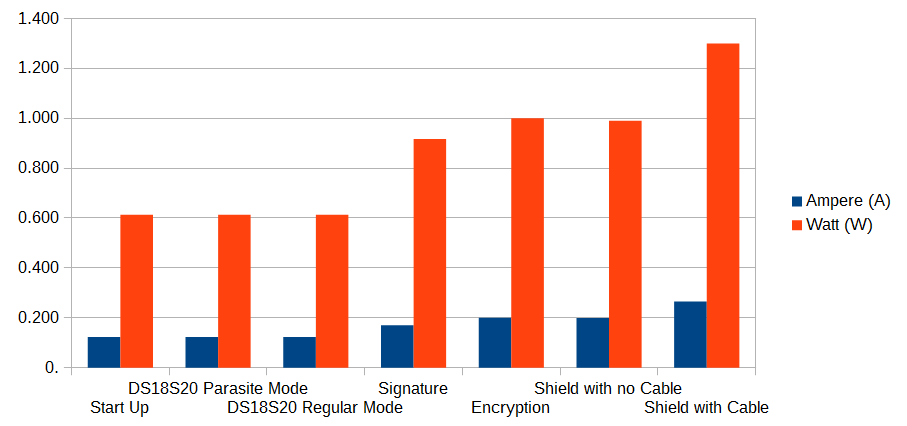
\includegraphics[width=1.1\linewidth]{Figures/power.png}
	\caption{Asymmetric Key Encryption}
	\label{fig:power}
\end{figure}


To start, the power was recorded as the temperature was being taken with the DS18S20 temperature sensor, in both parasite power mode and regular power mode. It was found that during both operations the power consumption was the exact same at 0.123A and 0.613W. This result was not surprising as the power consumption of the temperature sensor is so small compared to the Due that when the consumption of regular power mode and parasite mode are compared, there is little to no difference.

To isolate the the power consumed when the Due was only signing and encrypting, the Ethernet shield was left unplugged. This way the effect of the encryption would be seen without the effects of powering an Ethernet shield throughout. 
The readings upon start up were 0.123A and 0.613W, when the data was being given a signature the readings were 0.17A and 0.970W and when the message was encrypted it rose to 0.20A and 1W. 

In addition the power consumption when the Ethernet shield was attached but had no cable plugged was recorded. The power consumed during the signature and encryption process was the same as above but during DCHP the readings were 0.199A and 0.990W as it tried to gain an IP address from the router. Once the loop iteration was complete, the code went straight into a busy loop which was a tiny drop in power at 0.198A and 0.980W. A busy wait is a waste of power and resources so at this point the Arduino Due should go into a sleep mode and be woken up by an interrupt when it was to record the temperature again. 

The next test was with the shield plugged in and connected to the router with the Ethernet cable. The power consumption shot up to 0.265A and 1.30W during DHCP at the start of the sketch and there it remained even during the encryption process. Evidently the shield requires such a significant amount of the power that by comparison the cryptographic library is as good as unnoticeable. There are versions of the Ethernet Shield with an extra module that allows power over Ethernet. This extra module doesn't add a significant increase to the overall cost to the shield but can alleviate battery problems and extend the life of batteries by extracting power from the Ethernet cable that is connected to the router
%voltage changes??

The final test was to find out if there was a difference in power consumption depending on the length of message sent. Messages of size 20 and size 250 were sent with no appreciable difference in power consumption found.


The voltage through the experiments was the exact same, a steady 4.96V which makes sense as this is round about what USB 2.0 can give out and is well within normal limits for the Arduino Due.


%is flashed the normal way
%take temp reading every couple of seconds in parasite mode, 
%4.96V, 0.123A, 613mW
%flashed through device with empty code
%power reading stay same
%flashed normally with empty code
%same
%flashed normal and not
%take temp reading every couple of seconds in parasite mode
%same again
%During the dhcp and connecting to server .199A and 990mW with no ethernet plugged in
%During the busy wait at the end of loop delay() the current is .198A and 980mW a tiny drop in current
%with ethernet plugged in, sending encrypted data
%1.30w /0.265a
%tested on data of 19 length and 209, made no difference
%with ethernet plugged in but no encryption
%1.30w /0.265a


\section{Additional Objectives}

\subsection{Transmission of public keys}

Expansion of the network was considered with multiple devices communicating directly. This objective was reached by adding an Arduino Uno with another Ethernet shield as a webserver and the Due could pass on data, such as new server public keys, to it. If more nodes where desired then more Uno webservers could be added, the Due would simply go through the list of servers and send a POST request to each one to update their keys. At present the Due passes on the server's public key that it receives when it receives it. 

\subsection{Secure Transmission of Nonces}

Instead of using nonces that can be predicted, say counters, this application encrypts and sends the nonce to be used in the next temperature data transmission using the nonce from the previous data transmission or in the initial case a pre-installed nonce, which is never used again. The nonces are created randomly on the server and then sent securely, this ensures that the nonce for the secure temperature data transmission can never be guessed and the system is protected against replay attacks.

%\subsection{rekeying on arduino}
%http://blog.skylable.com/2014/05/tweetnacl-carrybit-bug/